\documentclass[12pt]{article}

\usepackage[utf8]{inputenc}
\usepackage[danish]{babel}
\usepackage{latexsym, amsfonts, amssymb, amsthm, amsmath, siunitx, graphicx, pgfplots}
\usepackage{fancyhdr, lastpage}

%loaded last
\usepackage[hidelinks]{hyperref}


\sisetup{exponent-product = \cdot,
  output-decimal-marker = {,}}

%Giles Castelles incfig
\usepackage{import}
\usepackage{xifthen}
\usepackage{pdfpages}
\usepackage{transparent}

\newcommand{\incfig}[2][1]{%
  \def\svgwidth{#1\columnwidth}
  \import{../figures/}{#2.pdf_tex}
}

\pdfsuppresswarningpagegroup=1

\setlength{\parindent}{0in}
\setlength{\oddsidemargin}{0in}
\setlength{\textwidth}{6.5in}
\setlength{\textheight}{8.8in}
\setlength{\topmargin}{0in}
\setlength{\headheight}{18pt}

\pgfplotsset{compat=newest}

\pgfplotsset{every axis/.append style={
  axis x line=middle,    % put the x axis in the middle
  axis y line=middle,    % put the y axis in the middle
  axis line style={<->,color=black}, % arrows on the axis
}}

\title{Opgaver til forelæsning 10}
\author{Noah Rahbek Bigum Hansen}
\date{12. Oktober 2024}

\begin{document}

\maketitle

\section*{Opg. 7.4}
The \textit{food calorie}, equal to \qty{4186}{J}, is a measure of how much energy is released when the body metabolizes food. A certain fruit-and-cereal bar contains \num{140} food calories. 

\subsection*{(a)}
If a \qty{65}{kg} hiker eats one bar, how high a mountain must he climb to “work off” the calories, assuming that all the food energy goes into increasing gravitational potential energy?
\bigbreak
Den samlede energi i myslibaren findes som
\[
  E_{mysli} = \qty{140}{kCal} \cdot \qty{4186}{\frac{J}{kCal}} = \qty{586040}{J}
.\] 
Den potentielle energi i tyngdefeltet er givet ved
\[
U_t = m\cdot g\cdot h \implies h = \frac{U_t}{m\cdot g} = \frac{\qty{586040}{J}}{\qty{65}{kg}\cdot \qty{9,81}{\frac{m}{s^2}}} = \qty{0,92}{km}
.\]

\subsection*{(b)}
If, as is typical, only \num{20}\% of the food calories go into mechanical energy, what would be the answer to part (a)? (\textit{Note}: In this and all other problems, we are assuming that \num{100}\% of the food calories that are eaten are absorbed and used by the body. This is not true. A person’s “metabolic efficiency” is the percentage of calories eaten that are actually used; the body eliminates the rest. Metabolic efficiency varies considerably from person to person.)
\bigbreak
Hvis kun 20\% af energien optages må vi have at klatreren kan bevæge sig 20\% af distancen fra før. Altså fås at
\[
h_{20\%} = h\cdot 20\% = \qty{0,92}{km}\cdot 20\% = \qty{0,18}{km}
.\] 
  

\section*{Opg. 7.9}

\begin{figure} [ht]
  \centering
  \caption{}
  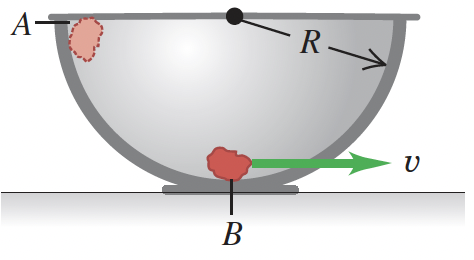
\includegraphics[width=0.5\linewidth]{../figures/E7_9.png}
  \label{fig:E7_9}
\end{figure}

A small rock with mass \qty{0,20}{kg} is released from rest at point $A$, which is at the top edge of a large, hemispherical bowl with radius $R = \qty{0,50}{m}$ (\textbf{\autoref{fig:E7_9}}). Assume that the size of the rock is small compared to $R$, so that the rock can be treated as a particle, and assume that the rock slides rather than rolls. The work done by friction on the rock when it moves from point $A$ to point $B$ at the bottom of the bowl has magnitude \qty{0,22}{J}.

\subsection*{(a)}
Between points $A$ and $B$, how much work is done on the rock by

\subsubsection*{(i)}
the normal force and
\bigbreak
The normal force is always perpendicular to the direction in which the stone is travelling, thus the normal force can at no point do any work.

\subsubsection*{(ii)}
gravity?
\bigbreak
The work done by gravity is opposite the change in the potential energy of the rock. Thus we have
\[
W_g = -\Delta U_t = -m\cdot g\cdot \Delta h = -\qty{0,20}{kg}\cdot \qty{9,81}{\frac{m}{s^2}}\cdot \qty{0,50}{m} = \qty{0,981}{J}
.\] 

\subsection*{(b)}
What is the speed of the rock as it reaches point $B$?
\bigbreak
Den kinetiske energi er summen af alt arbejdet udført på stenen. Friktionens arbejde må være modsatrettet stenens bevægelsesretning og tyngdekraftens arbejde må være i samme retning og det samlede arbejde må derfor være 
\[
k = W_{tot} = W_t - W_\mu
.\] 
Dermed kan hastigheden beregnes som
\[
v = \sqrt{\frac{2k}{m}} = \sqrt{\frac{2\cdot \left( \qty{0,981}{J} - \qty{0,22}{J} \right) }{\qty{0,20}{kg}}} = \qty{2,76}{\frac{m}{s}} 
.\] 


\subsection*{(c)}
Of the three forces acting on the rock as it slides down the bowl, which (if any) are constant and which are not? Explain.
\bigbreak
Tyngdekraften er konstant, men normalkraften er ikke, da den afhænger af skålens vinkel og da gnidningskraften afhænger af normalkraften er den ej heller konstant.


\subsection*{(d)}
Just as the rock reaches point $B$, what is the normal force on it due to the bottom of the bowl?
\bigbreak
Idet stenen netop når punkt B vil den opleve en normalkraft der modsvarer summen af de andre kræfter stenen oplever. Disse andre kræfter er hhv. tyngdekraften og centripetalkraften. Altså har vi
\[
F_N = -(F_t + F_c) = -m(g + \frac{v^2}{r}) = - \qty{0,20}{kg}\left( \qty{-9,81}{\frac{m}{s^2}} + \frac{(\qty{-2,76}{\frac{m}{s}})^2}{\qty{0,50}{m}} \right) = \qty{5,0}{N} 
.\] 

\section*{Opg. 7.19}
A spring of negligible mass has force constant $k = \qty{800}{\frac{N}{m}}$.

\subsection*{(a)}
How far must the spring be compressed for \qty{1,20}{J} of potential energy to be stored in it?
\bigbreak
Formlen for en fjeders potentielle energi er
\[
U_s = \frac{1}{2}kx^2
.\] 
Heri kan strækningen, $x$, isoleres som så
\[
x = \sqrt{\frac{2U_s}{k}} = \sqrt{\frac{2\cdot \qty{1,20}{J}}{\qty{800}{\frac{N}{m}}}} = \qty{5,48}{cm}
.\] 

\subsection*{(b)}
You place the spring vertically with one end on the floor. You then lay a \qty{1,60}{kg} book on top of the spring and release the book from rest. Find the maximum distance the spring will be compressed.
\bigbreak
Fjederen vil blive trykket sammen netop indtil arbejdet udøvet på fjederen netop har samme størrelse som tyngdekraftens arbejde. Altså har vi at
\[
|W_t| = |U_s| \implies m\cdot g\cdot x = \frac{1}{2} k\cdot x^2 \implies x = \frac{2m\cdot g}{k} = \frac{2\cdot \qty{1,60}{kg}\cdot \qty{9,81}{\frac{m}{s^2}}}{\qty{800}{\frac{N}{m}}} = \qty{3,92}{cm}
.\] 


\section*{Opg. 7.29}
A \qty{62,0}{kg} skier is moving at \qty{6,50}{m/s} on a frictionless, horizontal, snow-covered plateau when she encounters a rough patch \qty{4,20}{m} long. The coefficient of kinetic friction between this patch and her skis is \num{0,300}. After crossing the rough patch and returning to friction-free snow, she skis down an icy, frictionless hill \qty{2,50}{m} high.

\subsection*{(a)}
How fast is the skier moving when she gets to the bottom of the hill?
\bigbreak
Først regnes arbejdet som friktionskraften har udført på skiløberen. Her har vi at
\[
W_\mu = F_\mu \cdot s = F_N \cdot \mu \cdot s = m\cdot g \cdot \mu \cdot s = \qty{62,0}{kg}\cdot \qty{9,81}{\frac{m}{s^2}}\cdot \num{0,300}\cdot \qty{4,20}{m} = \qty{766,357}{J}
.\] 
Dernæst kan arbejdet som tyngdekraften har udført på hende på det sidste stykke regnes. Denne er givet ved
\[
W_t = m\cdot g\cdot h = \qty{62,0}{kg}\cdot \qty{9,81}{\frac{m}{s^2}}\cdot \qty{2,50}{m} = \qty{1520,55}{J}
.\] 
Det samlede tilførte arbejde er altså
\[
W_{tot} = W_t - W_\mu = \qty{1520,55}{J} - \qty{766,357}{J} = \qty{754,193}{J}
.\] 
Hendes kinetiske energi før var hun ramte stykket med friktion var
\[
k_0 = \frac{1}{2}m\cdot v_0^2 = \frac{1}{2}\cdot \qty{62,0}{kg}\cdot \left( \qty{6,50}{\frac{m}{s}} \right)^2 = \qty{1309,75}{J}
.\] 
Og hendes samlede kinetiske energi i bunden af bakken er derfor
\[
k_{tot} = k_0 + W_{tot} = \qty{2063,943}{J}
,\] 
Hvilket svarer til en hastighed på
\[
v = \sqrt{\frac{2k_{tot}}{m}} =  \sqrt{\frac{2\cdot \qty{2063,943}{J}}{\qty{62,0}{kg}}} = \qty{8,16}{\frac{m}{s}}
.\] 

\subsection*{(b)}
How much internal energy was generated in crossing the rough patch?
\bigbreak
Dette er fundet som $W_\mu = \qty{766}{J}$ i opgaven ovenfor
  

\section*{Opg. 7.32}
The potential energy of a pair of hydrogen atoms separated by a large distance $x$ is given by $U(x) = -\frac{C_6}{x^6}$, where $C_6$ is a positive constant. What is the force that one atom exerts on the other? Is this force attractive or repulsive?
\bigbreak
Idet vi ved at $U = \int F \, \mathrm{d}s$ må det gælde at
\[
F = - \frac{\mathrm{d}U}{\mathrm{d}x} 
.\] 
Altså har vi
\[
F = -6C_6\cdot x^{-7}
.\]
Af det oprindelige udtryk for den potentielle energi kan ses at hvis afstanden mellem de to atomer, $x$, øges så stiger den potentielle energi og derfor må de to hydrogenatomer tiltrække hinanden.


\section*{Opg. 7.37}

\begin{figure} [ht]
  \centering
  \caption{}
  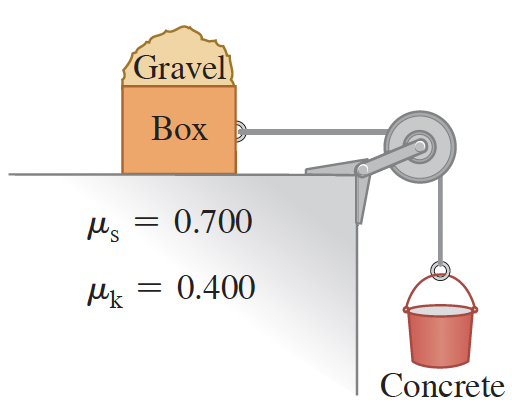
\includegraphics[width=0.5\linewidth]{../figures/P7_37.png}
  \label{fig:P7_37}
\end{figure}

At a construction site, a \qty{65,0}{kg} bucket of concrete hangs from a light (but strong) cable that passes over a light, friction-free pulley and is connected to an \qty{80,0}{kg} box on a horizontal roof (\textbf{\autoref{fig:P7_37}}). The cable pulls horizontally on the box, and a \qty{50,0}{kg} bag of gravel rests on top of the box. The coefficients of friction between the box and roof are shown.

\subsection*{(a)}
Find the friction force on the bag of gravel and on the box.
\bigbreak
Den maksimale friktionskraft, $F_{\mu_max}$ er givet ved
\[
  F_{\mu_max} = F_N\cdot \mu = m\cdot g\cdot \mu = (\qty{80,0}{kg} + \qty{50,0}{kg})\cdot \qty{9,81}{\frac{m}{s^2}}\cdot \num{0,700} = \qty{892,71}{N}
.\] 
Friktionskraften er dog kun så stor som den kraft der trækker i kassen, $T$
 \[
T = w_c = m_c \cdot g = \qty{65,0}{kg}\cdot \qty{9,81}{\frac{m}{s^2}} = \qty{638}{N}
.\] 


\subsection*{(b)}
Suddenly a worker picks up the bag of gravel. Use energy conservation to find the speed of the bucket after it has descended 2.00 m from rest. (Use Newton’s laws to check your answer.)
\bigbreak
Vi har at
\[
k_1 + U_1 + W_\mu = k_2 + U_2 \implies 0 + m_c\cdot g\cdot s + (- m_b\cdot g\cdot \mu_k\cdot s) = \frac{1}{2}(m_b + m_c)v^2
.\] 
Altså har vi at
\[
v = \sqrt{\left( \frac{2(m_c - m_b\mu_k)sg}{m_b + m_c} \right) } = \sqrt{\left( \frac{2\cdot (\qty{65,0}{kg} - \qty{80,0}{kg}\cdot \num{0,400})\qty{2,00}{m}\cdot \qty{9,81}{\frac{m}{s^2}}}{\qty{65,0}{kg}+\qty{80,0}{kg}} \right) } = \qty{2,99}{\frac{m}{s}} 
.\] 


  

\section*{Opg. 7.41}

\begin{figure} [ht]
  \centering
  \caption{}
  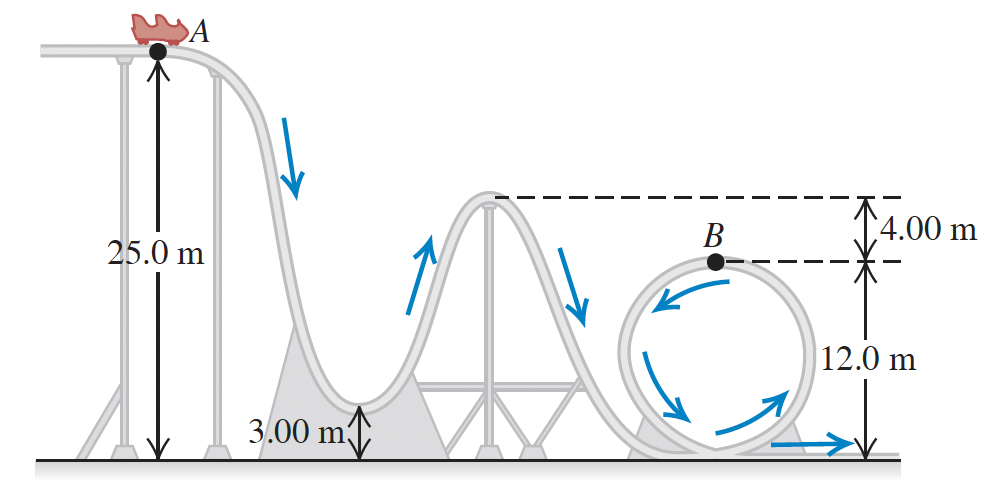
\includegraphics[width=0.5\linewidth]{../figures/P7_41.png}
  \label{fig:P7_41}
\end{figure}

A \qty{350}{kg} roller coaster car starts from rest at point $A$ and slides down a frictionless loop-the-loop (\textbf{\autoref{fig:P7_41}}) . The car’s wheels are designed to stay on the track.

\subsection*{(a)}
How fast is this roller coaster car moving at point $B$?
\bigbreak
Til punktet $B$ har rutsjebanen bevæget sig sammenlagt $\qty{25,0}{m} - \qty{12,0}{m} = \qty{13,0}{m}$ ned i tyngdefeltet. Altså er den kinetiske energi her
\[
k = \Delta U_t = m\cdot g\cdot h = \qty{350}{kg}\cdot \qty{9,81}{\frac{m}{s^2}}\cdot \qty{13,0}{m} = \qty{44,636}{kJ}
.\] 
Dette tilsvarer en hastighed på
\[
v = \sqrt{\frac{2k}{m}} = \sqrt{\frac{2\cdot \qty{44,636}{kJ}}{\qty{350}{kg}}} = \qty{15,97}{\frac{m}{s}}
.\] 

\subsection*{(b)}
How hard does it press against the track at point $B$?
\bigbreak
Normalkraften til punktet $B$ er givet som differensen mellem centripetalkraften her og tyngdekraften. Altså har vi
 \[
F_N = F_c - F_t \implies F_N = m \frac{v^2}{r} - mg = m\left(\frac{v^2}{r}-g\right) .\] 

\[
  F_N = \qty{350}{kg}\left( \frac{\left( \qty{15,97}{\frac{m}{s}} \right)^2 }{\qty{6,0}{m}} - \qty{9,81}{\frac{m}{s^2}} \right) = \qty{11,4}{kN} 
.\] 

\section*{Opg. 7.50}

\begin{figure} [ht]
  \centering
  \caption{}
  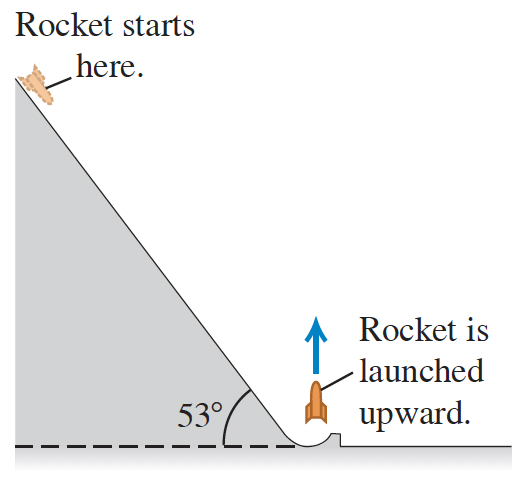
\includegraphics[width=0.5\linewidth]{../figures/P7_50.png}
  \label{fig:P7_50}
\end{figure}

A \qty{1500}{kg} rocket is to be launched with an initial upward speed of \qty{50,0}{m/s}. In order to assist its engines, the engineers will start it from rest on a ramp that rises \ang{53} above the horizontal (\textbf{\autoref{fig:P7_50}}). At the bottom, the ramp turns upward and launches the rocket vertically. The engines provide a constant forward thrust of \qty{2000}{N}, and friction with the ramp surface is a constant \qty{500}{N}. How far from the base of the ramp should the rocket start, as measured along the surface of the ramp?
\bigbreak
Først findes den kinetiske energi der er påkrævet for at opnå den ønskede affyringshastighed. Dette gøres som
\[
k = \frac{1}{2}\cdot m\cdot v^2 = \frac{1}{2}\cdot \qty{1500}{kg}\cdot \left( \qty{50,0}{\frac{m}{s}} \right)^2 = \qty{1875000}{J}
.\] 
Denne kinetiske energi må være givet ved
\[
k = W_t + W_{rocket} + W_\mu
.\] 
Først kan tyngdekraftens arbejde findes som
\[
  U_t = m\cdot g\cdot h = m\cdot g\cdot \sin{\alpha} \implies W_t = m\cdot g\cdot \sin(\alpha)\cdot s
.\] 
Rakettens arbejde må være
\[
W_{rocket} = F_{rocket} \cdot s
.\] 
Og friktionskraftens arbejde må være
\[
W_\mu = F_{\mu} \cdot s
.\] 
Altså har vi at
\[
k = m \cdot g \cdot s \cdot \sin(\alpha) + F_{rocket} \cdot s + F_\mu \cdot s = s\left( m\cdot g\cdot \sin(\alpha) + F_{rocket} + F_mg \right) 
.\]
Strækningen kan isoleres
\[
s = \frac{k}{m\cdot g\cdot \sin(\alpha)+F_{rocket}+F_{\mu}} = \frac{\qty{1875000}{J}}{\qty{1500}{kg}\cdot \qty{9,81}{\frac{m}{s^2}\cdot \sin(\ang{53}) + \qty{2000}{N} \qty{-500}{N}}} = \qty{141}{m}
.\]



\section*{Opg. 7.59}
A certain spring found \textit{not} to obey Hooke’s law exerts a restoring force $F_x(x) = -\alpha x - \beta x^2$ if it is stretched or compressed,
where $\alpha = \qty{60,0}{\frac{N}{m}}$ and $\beta = \qty{18.0}{\frac{N}{m^2}}$. The mass of the spring is negligible. 


\subsection*{(a)}
Calculate the potential-energy function $U(x)$ for this spring. Let $U = 0$ when $x = 0$.
\bigbreak
Vi ved at
\[
U(x) = \int F_x (x) \, \mathrm{d}x = \frac{1}{2}\alpha x^2 +\frac{1}{3}\beta x^3 + c
.\] 
Og
\[
U(0) = 0 \implies c=0
.\]
Altså har vi at
\[
U(x) = \frac{1}{2}\alpha x^2 + \frac{1}{3} \beta x^3
.\] 


\subsection*{(b)}
An object with mass \qty{0,900}{kg} on a frictionless, horizontal surface is attached to this spring, pulled a distance \qty{1,00}{m} to the right (the $+x$-direction) to stretch the spring, and released. What is the speed of the object when it is \qty{0,50}{m} to the right of the $x = 0$ equilibrium position?
\bigbreak
Først findes den potentielle energi lagret i fjederen i yderpositionen som
\[
U(\qty{1,00}{m}) = \frac{1}{2}\cdot \qty{60,0}{\frac{N}{m}}\cdot (\qty{1,00}{m})^2 + \frac{1}{3}\cdot \qty{18,0}{\frac{N}{m^2}}\cdot (\qty{1,00}{m})^3 = \qty{36}{J}
.\]
Og dernæst kan det samme gøres for $U(\qty{0,50}{m})$
\[
U(\qty{0,50}{m}) = \frac{1}{2}\cdot \qty{60,0}{\frac{N}{m}}\cdot (\qty{0,50}{m})^2 + \frac{1}{3}\cdot \qty{18,0}{\frac{N}{m^2}}\cdot (\qty{1,00}{m})^3 = \qty{8,25}{J}
.\] 
Altså må den samlede kinetiske energi af objektet være
\[
k = U(\qty{1,00}{m}) - U(\qty{0,50}{m}) = \qty{36}{J} - \qty{8,25}{J} = \qty{27,75}{J}
.\] 
Dette svarer til en hastighed på
\[
v = \sqrt{\frac{2k}{m}} = \sqrt{\frac{2\cdot \qty{27,75}{J}}{\qty{0,900}{kg}}} = \qty{7,85}{\frac{m}{s}}
.\] 


\end{document}
